\documentclass[pdflatex,sn-basic]{sn-jnl}

% ---- packages ---------------------------------------------------------------
%  sn-jnl.cls already provides hyperref, natbib, url and the caption setup;
%  do not load those again or you will get an option clash.
\usepackage{graphicx}
\graphicspath{{assets/}}% figures live in assets/figures/; includes stay figures/...
\usepackage{amsmath,amssymb,amsfonts,bm}
\usepackage{booktabs}
\usepackage{array}
\usepackage{tabularx}
\usepackage{ragged2e}

% ---- column types used by the differentiation matrices (Tables 5 and 6) ------
\newcolumntype{L}[1]{>{\RaggedRight\arraybackslash\hspace{0pt}}p{#1}}
\newcolumntype{Y}{>{\RaggedRight\arraybackslash\hspace{0pt}}X}

\renewcommand{\arraystretch}{1.15}
\setlength{\emergencystretch}{1.5em}

\begin{document}

% ============================== TITLE BLOCK =================================
\title[Hamiltonian Vision Kernel]{Hamiltonian Vision Kernel: Symmetry-Pooled
  Quantum Correlator Features with Hardware Validation}

\author[1]{\fnm{Sparsho} \sur{Chakraborty}}\email{25ph05023@iitbbs.ac.in}

\author*[2]{\fnm{Siddhartha} \sur{Patra}}\email{siddhartha.patra@tcgcrest.org}

\affil[1]{\orgdiv{School of Basic Sciences, Department of Physics},
  \orgname{Indian Institute of Technology Bhubaneswar},
  \orgaddress{\state{Odisha}, \country{India}}}

\affil*[2]{\orgdiv{Centre for Quantum Engineering, Research and Education},
  \orgname{TCG CREST}, \orgaddress{\city{Kolkata}, \country{India}}}

% ---- abstract: 230 words (QMI requires 150-250) ------------------------------
\abstract{We introduce the Hamiltonian Vision Kernel (HVK), a hybrid quantum--classical
architecture for image reconstruction. HVK assembles matrix-product-state patch
features, a variational quantum circuit exposing a Pauli-correlator latent
space, two-dimensional Fourier positional encoding, a learnable Hamiltonian
energy diagnostic, and a classical decoder into a single pipeline. Two
instantiations, HVK1D and HVK2D, realise chain and grid interaction graphs;
group-averaged observable pooling makes the HVK2D feature map exactly
equivariant to the eight symmetries of the square. The contribution is this
specific assembly rather than any ingredient in isolation. Across six real image
datasets, per-image-trained HVK2D models reconstruct with peak signal-to-noise
ratio (PSNR) between 25.8 and 41.6 decibels. On a resource-matched, multi-seed
held-out comparison using the CIFAR-10 image dataset, a pre-declared two
one-sided tests (TOST) equivalence procedure at a one-decibel margin establishes
that HVK2D is statistically \emph{competitive} with resource-matched
local-observable and raw-linear classical controls, and it substantially
outperforms random-circuit and classical-random-feature controls. Five fitted checkpoints
are replayed on superconducting quantum hardware without retraining and decoded
directly from device-measured observables, reaching 25.90 to 31.52 decibels. The
capabilities that a purely classical reconstruction pipeline does not natively
provide are an entangling observable channel that is representationally
necessary on a leakage-audited task requiring distant-patch products, an
interpretable Hamiltonian energy diagnostic, and native execution on quantum
hardware. We make no claim of quantum advantage.}

% ---- keywords: 6 (QMI requires 4-6) -----------------------------------------
\keywords{Quantum image processing, Tensor networks, Variational quantum
  algorithms, Pauli observables, Group-equivariant representations,
  Quantum hardware validation}

\maketitle

% ================================ BODY ======================================
\section{Introduction}
\label{sec:intro}

Hybrid quantum--classical models for vision tasks are increasingly proposed as a
route to representations with favorable inductive bias, exploiting entanglement,
physically motivated regularizers, or tensor-network structure that classical
convolutional pipelines do not natively expose
\citep{Cerezo2021, Tilly2022, Preskill2018}. The variational quantum eigensolver
and its descendants exploit the local decomposability of physically relevant
Hamiltonians to construct shallow, problem-aware circuits
\citep{Cerezo2021, Tilly2022, Bauer2020}, and quantum image processing provides
encodings that place pixel information directly into qubit registers, from
flexible amplitude-style representations \citep{Le2011} to basis-encoded pixel
values \citep{Zhang2013} and their processing primitives
\citep{Chakraborty2018, Zhou2017, Yao2017}. Tensor-network methods, in parallel,
have proven effective as compressed representations of structured classical
data, including images
\citep{Cirac2021, Latorre2005, Han2018, Stoudenmire2016, Ran2020TNCS, Guala2023},
and more broadly other structured data such as particle-physics events
\citep{Araz2022}. Related hybrid quantum architectures target adjacent imaging
tasks, including quantum annealing-based tomographic reconstruction
\citep{Haga2024}, adiabatic quantum computing for emission tomography
\citep{Nau2023}, quantum neural compressive sensing for ghost imaging
\citep{Zhai2025}, hybrid autoencoder-plus-quantum-SVM feature extraction for
image classification \citep{Slabbert2024}, quantum convolutional networks and
their classical-data variants \citep{Cong2019, Hur2022}, and quantum capsule
networks \citep{Liu2022}. HVK focuses on the specific combination of a
Pauli-correlator latent space, enforced group-equivariant pooling, and a
physically motivated energy diagnostic.

We introduce the Hamiltonian Vision Kernel (HVK1D/HVK2D), which combines these
ingredients into a single architecture with three properties studied jointly
here: a \emph{Pauli-correlator latent space} (measured VQC observables, not a raw
quantum state, form the representation handed to a classical decoder, in the
spirit of quantum-enhanced feature maps \citep{Havlicek2019}); an \emph{exact,
numerically-verified $D_4$-equivariant observable-pooling construction},
group-averaging the observable grid over the eight symmetries of the square
rather than merely motivating symmetry through architecture choices, in the
spirit of group-equivariant classical vision \citep{Cohen2016, Bronstein2021}
and the equivariant-quantum-neural-network line that formalizes
symmetry-embedding constructions for variational circuits
\citep{Meyer2023, Nguyen2024EQNN, Schatzki2024, West2024, West2024Erratum}; and a
\emph{learnable Hamiltonian energy diagnostic} (full nearest-neighbor
$XX/YY/ZZ$ sectors in HVK1D and grid-edge $ZZ$ terms in HVK2D).
Table~\ref{tab:differentiation} contrasts these properties against classical,
adversarial, and standard quantum autoencoder baselines.

\subsection*{Novelty relative to the nearest hybrid-vision architectures}

HVK's closest architectural relatives are three hybrid quantum-vision patterns
already established individually in the literature, and situating HVK against
each clarifies what is new here versus what is inherited.
\emph{Register-based quantum autoencoders}
\citep{Romero2017, WangQAECompression2024, QAEClassification2025} encode an
image's pixel amplitudes directly into a qubit register and train a trash-qubit
fidelity objective (or attach a classical decoder to that register's measured
amplitudes); HVK never amplitude-encodes pixels into qubits at all --- it
exposes only classically pre-compressed MPS patch features as circuit input, and
hands the decoder measured Pauli correlators rather than register amplitudes or a
fidelity score. \emph{Quantum-kernel vision models}
\citep{Havlicek2019, QuantumKernelDefect2022} embed an input into a quantum
feature space and read out a scalar kernel (state-overlap) value consumed by a
classical kernel method; HVK instead reads out an explicit vector of local and
pairwise Pauli expectation values as a latent representation for a trained
decoder, and adds enforced group-equivariant pooling and a Hamiltonian
regularizer that a kernel construction has no analogue for.
\emph{Tensor-network (TN) circuit classifiers}
\citep{Guala2023, Stoudenmire2016, Han2018} use MPS structure either as a
standalone classical model or as a template for a shallow quantum circuit trained
for classification; HVK uses MPS compression only as a classical
\emph{preprocessing} step that sets a separately trained VQC's rotation angles,
and targets per-image reconstruction rather than classification. None of these
three families combines classical MPS-compressed input, a measured
Pauli-correlator (not kernel- or register-state) latent space, enforced
$D_4$-equivariant pooling, and a learnable Hamiltonian diagnostic in one
pipeline; HVK's contribution is this specific \emph{assembly} and the properties
it jointly enables (Table~\ref{tab:differentiation}), not any single ingredient in
isolation --- each of which individually recurs throughout this literature
(Section~\ref{sec:representativeness}).

\subsection*{Contributions}

\begin{enumerate}\itemsep3pt
  \item \textbf{Architecture.} HVK1D/HVK2D combines MPS patch features, a
        six-qubit VQC, a 19--27-dimensional Pauli-correlator vector, 2D Fourier
        positional encoding, a graph-Hamiltonian diagnostic, and a classical
        decoder.
  \item \textbf{Reconstruction scope.} Identically configured per-image fitting
        experiments cover six real image datasets
        (Section~\ref{sec:sameset_results}).
  \item \textbf{Competitive with resource-matched classical baselines.} A
        pre-declared TOST equivalence test on held-out CIFAR-10 shows HVK2D is
        statistically equivalent, within a $\pm1$~dB margin, to six of eight
        resource-matched classical/ablated controls, and substantially
        outperforms the two null controls (strict classical random features and
        a random-VQC) (Section~\ref{sec:ablation_relationship}).
  \item \textbf{Hardware pilot.} Five fitted checkpoints are replayed on IBM
        hardware without retraining and decoded from hardware-measured
        observables (Section~\ref{sec:hardware_pilot}), strengthened by a
        noise/shot-budget sweep and repeated execution across backends
        (Sections~\ref{sec:hardware_robustness}--\ref{sec:hardware_anchors}).
  \item \textbf{Equivariant observable pooling.} An exact,
        numerically-verified $D_4$-equivariant observable-pooling construction
        makes the HVK2D observable map equivariant to the eight symmetries of
        the square, to floating-point precision (Section~\ref{sec:d4}). The
        guarantee follows from Reynolds group averaging over the $D_4$ orbit,
        not from anything quantum: the identical construction applied to a
        purely classical feature map yields the same exactness (Supplementary
        Material). We therefore report it as a property the assembled pipeline
        provides, not as a quantum result.
  \item \textbf{Restricted nonlocal result.} In a leakage-audited fixed-readout
        protocol, entangling pair observables are necessary when the target
        depends explicitly on distant-patch products
        (Section~\ref{sec:entanglement_necessity}).
\end{enumerate}

A companion document, \textit{Supplementary Material for the Hamiltonian Vision
Kernel: Resource-Matched Ablations, Validation, and Reproducibility}, reports
resource-matched held-out comparisons of HVK and classical/ablated feature maps,
together with full hardware-pilot methodology (circuit construction, validation,
job identifiers, quota accounting) and explicit provenance audits of excluded
exploratory results, among them the training-dynamics traces of
Section~\ref{sec:phase_transition}, which we report as an interpretability
readout rather than as evidence of a transition. We keep that analysis in a
companion document so the architecture-level contributions above and the
generalization question do not obscure each other;
Section~\ref{sec:ablation_relationship} summarizes its central finding and how it
relates to the results here.

\section{Hamiltonian Vision Kernel: Architecture}
\label{sec:architecture}

HVK treats each spatial patch as a finite spin state, compresses it as a matrix
product state (MPS), measures a fixed set of Pauli observables from a variational
quantum circuit (VQC), and decodes those observables back into pixels with a
classical multi-layer perceptron (MLP). A learnable graph-Hamiltonian energy term
regularizes training; unlike parameterized Hamiltonian learning approaches that
treat the Hamiltonian as the primary learned object \citep{Shi2022}, HVK's energy
term is a diagnostic regularizer alongside a separate reconstruction objective.

\paragraph{Problem statement.}
Given an image $x$ partitioned into non-overlapping patches
$\{x_p\}_{p=1}^{P}$, HVK learns a per-patch reconstruction map. Each patch is
compressed to a classical MPS feature vector $\phi_{\mathrm{MPS}}(x_p)$, a learned
linear layer sets the VQC rotation angles, and measuring a fixed set of Pauli
observables yields the correlator feature map
$\Phi(x_p)\in\mathbb{R}^{d}$ ($d=27$ for HVK1D, $19$ for HVK2D). A classical
decoder $D_\theta$ maps $\Phi(x_p)$, together with a Fourier positional encoding
$\pi(p)$, back to a reconstructed patch $\hat{x}_p=D_\theta\!\big(\Phi(x_p),\pi(p)\big)$.
Training minimizes the pixel-reconstruction loss with the graph-Hamiltonian energy
term $E(\cdot)$ as an auxiliary regularizer,
\begin{equation}
  \label{eq:objective}
  \mathcal{L}(\theta)=\sum_{p=1}^{P}\big\|x_p-\hat{x}_p\big\|_2^{2}
  \;+\;\lambda\,E\big(\Phi(x_p)\big),
\end{equation}
where $\lambda$ weights the diagnostic energy term (Section~\ref{sec:regularizer_inert}
reports its effect). The shared pipeline is
\begin{equation}
\begin{aligned}
\text{Image}
  &\rightarrow \{\text{Patches}\} \rightarrow \text{MPS}\\
  &\rightarrow \text{46-D/22-D Feature} \rightarrow \text{6-D Vector}\\
  &\rightarrow \text{27-D/19-D Latent} \rightarrow \text{Decoder}\\
  &\rightarrow \text{Reconstruction}.
\end{aligned}
\end{equation}

Three of these design choices warrant explicit motivation rather than being left
implicit in the pipeline above. \emph{Why MPS features}: treated as an
amplitude-encoded quantum state, a patch of $n$ sites has a coefficient tensor
with $2^{n}$ entries; matrix-product-state factorization instead represents it as
a chain of small tensors bounded by a fixed bond dimension $\chi$, a compact,
singular-value-controlled compression whose entanglement-entropy profile is
already known to track image compressibility
\citep{Latorre2005, Stoudenmire2016}, and whose local expectations and
correlations are cheap classical features rather than requiring a full
state-preparation circuit. \emph{Why a Pauli-correlator latent space rather than
a raw quantum state}: handing the classical decoder a fixed vector of measured
Pauli expectation values, instead of full state tomography, keeps the
quantum-to-classical interface at $O(\text{qubits})$ rather than exponential
readout cost and follows the same measured-observable-as-feature pattern used by
quantum-enhanced feature maps generally \citep{Havlicek2019}; it is also what
makes the interpretability diagnostics of Section~\ref{sec:regularizer_inert} and
the training-dynamics diagnostics reported in the companion Supplementary
Material possible, since a full state vector would not expose a comparably
compact, physically meaningful summary. \emph{Why a grid rather than chain
interaction topology for HVK2D}: aligning the six-qubit interaction graph with
the $2\times3$ patch-neighbor adjacency, rather than an arbitrary linear chain,
is what makes the $D_4$ group-pooling construction of Section~\ref{sec:d4}
well-defined in the first place --- the pooling operator averages over the
spatial symmetries of the square, which requires a latent structure that itself
respects the patch grid's two-dimensional adjacency. HVK1D's chain topology is
retained as the ungridded control this comparison needs
(Section~\ref{sec:topology}), not because a chain is separately motivated for 2D
image data.

Two executed preprocessing configurations share this pipeline. For the
$256\times256$ \textit{Monalisa}/HVK1D benchmark, sixteen non-overlapping
$64\times64$ patches are $\ell_2$-normalized, reshaped as 12-site spin states,
and sequentially SVD-compressed to MPS bond dimension $\chi=4$. Their 24 local
$X/Z$ expectations, 11 nearest-neighbor $ZZ$ correlations, and 11 bipartite
entropies form a 46-D feature vector. For the native $32\times32$ HVK2D
multi-dataset experiments, sixteen $8\times8$ patches are represented by six-site
MPSs, giving 12 local expectations, five nearest-neighbor $ZZ$ terms, and five
entropies (22 dimensions). A learned linear layer compresses either MPS feature
vector to six circuit angles. HVK1D then measures 27 observables (six local $Z$,
six local $X$, and five each of $ZZ$, $XX$, and $YY$); HVK2D measures 19 (six
local $Z$, six local $X$, and seven grid-edge $ZZ$ terms). The respective Fourier
positional vectors have dimension eight and four, following the established use
of Fourier positional encoding as a spatial inductive bias in classical
generative vision models \citep{Xu2021}. In both configurations, a
two-hidden-layer MLP (128 and 256 units) maps the observable and positional
vectors to one grayscale patch. Figure~\ref{fig:hvk_ansatz} shows the exact HVK1D
and HVK2D ansatz circuits (rebuilt in Qiskit and numerically verified against the
training-time PennyLane circuit as part of the hardware pilot of
Section~\ref{sec:hardware_pilot}); complete Hamiltonian, loss,
positional-encoding, and measurement definitions are retained in the companion
supplement.

\begin{figure}[t]
  \centering
  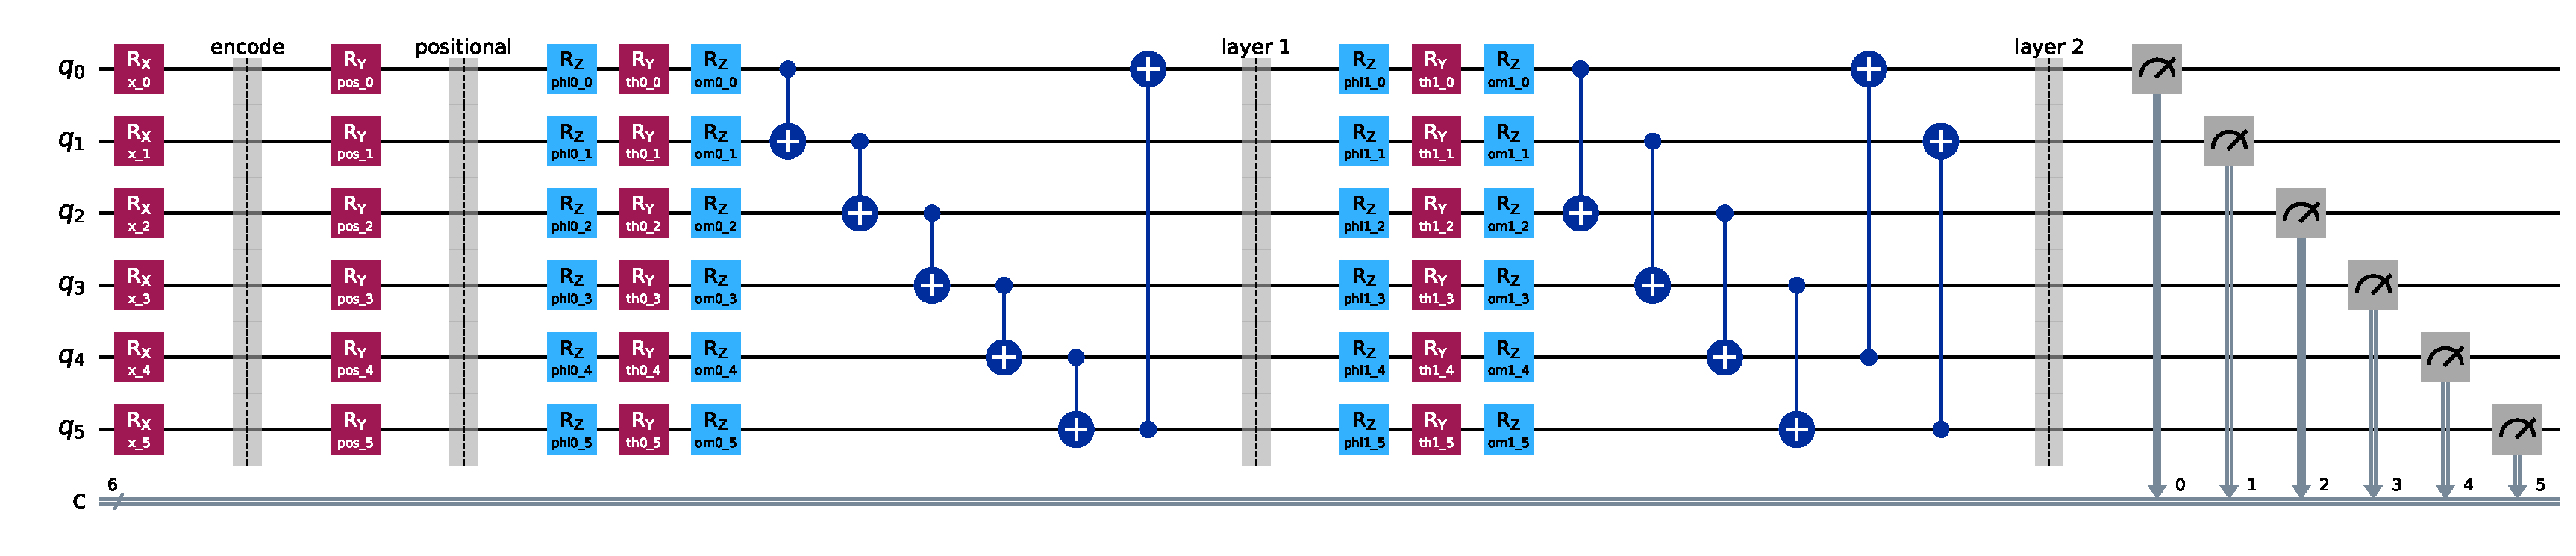
\includegraphics[width=\textwidth]{figures/hvk1d_ansatz.pdf}\\[6pt]
  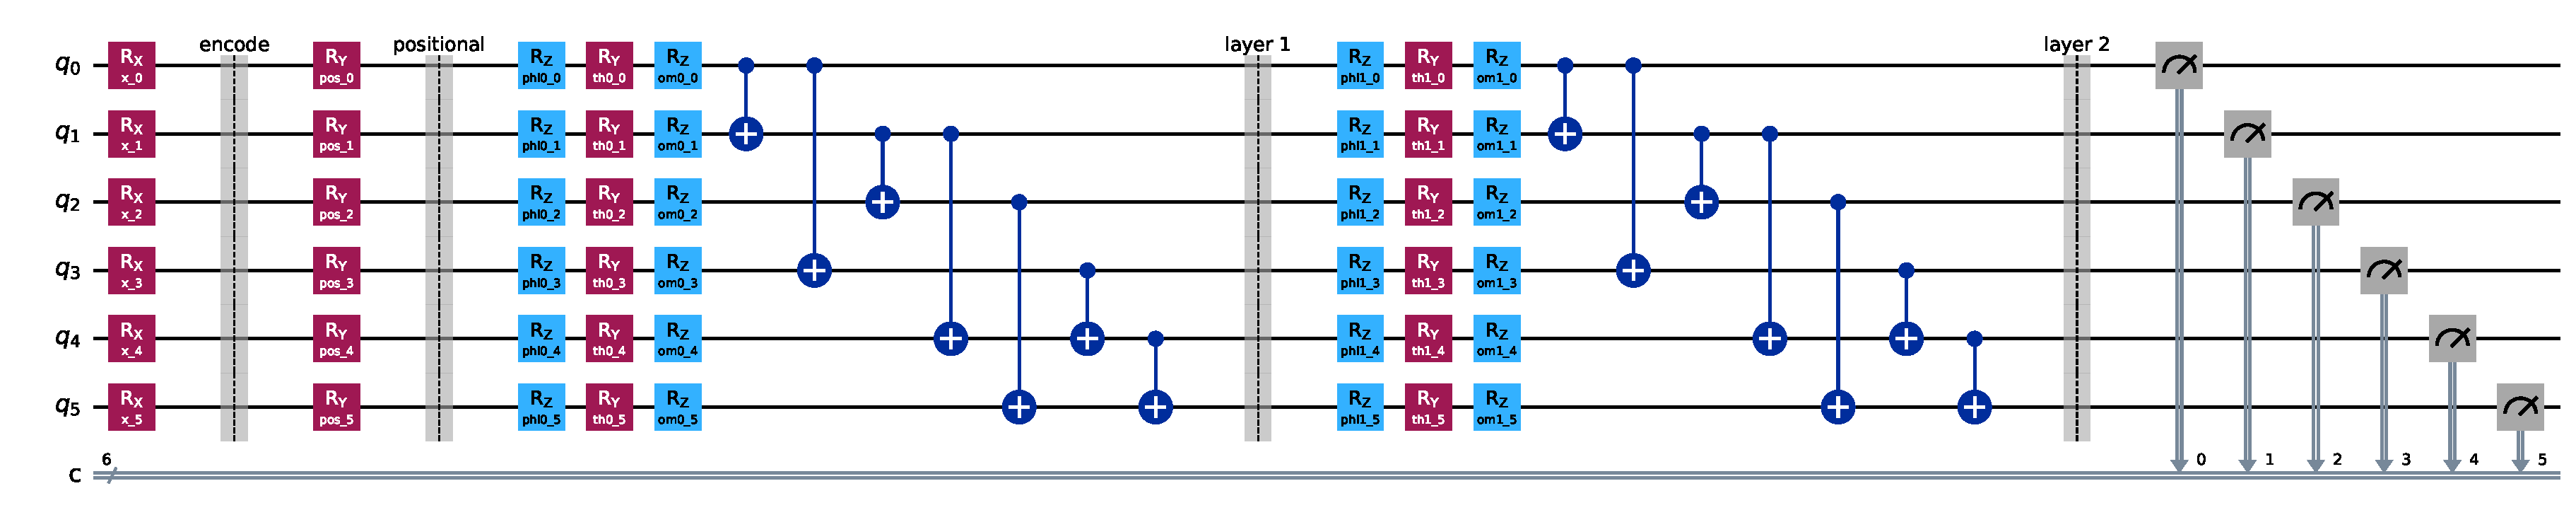
\includegraphics[width=\textwidth]{figures/hvk2d_ansatz.pdf}
  \caption{The HVK1D (top) and HVK2D (bottom) variational ans\"atze, exactly as
           executed (encoding $R_X$ rotations, positional $R_Y$ rotations, then
           two entangling layers of $R_Z$-$R_Y$-$R_Z$ single-qubit rotations with
           a CNOT ring for HVK1D or fixed grid-edge CNOTs for HVK2D). Both
           circuits were rebuilt gate-for-gate in Qiskit and validated against
           the original PennyLane training circuit before use in the hardware
           pilot of Section~\ref{sec:hardware_pilot}.}
  \label{fig:hvk_ansatz}
\end{figure}

Table~\ref{tab:variants} summarizes the tested variants. HVK1D uses a linear
6-qubit chain (5 nearest-neighbor bonds, 27-D observable vector); HVK2D arranges
the same 6 qubits on a $2\times3$ lattice matching patch-boundary adjacency
(19-D latent signature); a symmetric HVK1D variant adds a
$\mathrm{U}(1)$-preserving coupling constraint; and a $D_4$-pooled HVK2D variant
(Section~\ref{sec:symmetry}) group-averages the observable grid over the eight
symmetries of the square,
$\Phi_{D_4}(x)=\tfrac{1}{8}\sum_{g\in D_4}P_g^{-1}\Phi(gx)$, which is equivariant
by construction. The IBM Cloud circuit probe reported in the supplement confirms
both HVK1D and HVK2D compile to depth-18, 6-qubit circuits on a Heron-class
basis.

\begin{table}[t]
  \centering
  \caption{HVK variants tested in this paper.}
  \label{tab:variants}
  \begin{tabular}{@{}l l c l@{}}
    \toprule
    Variant                 & Topology                  & Latent dim. & Symmetry \\
    \midrule
    HVK1D                   & 6-qubit chain             & 27-D        & None (control)            \\
    HVK2D                   & $2\times3$ grid           & 19-D        & $D_4$-motivated only      \\
    Symmetric HVK1D         & 6-qubit chain             & 27-D        & $\mathrm{U}(1)$ coupling  \\
    $D_4$-pooled HVK2D      & $2\times3$ grid, pooled   & 19-D        & $D_4$-equivariant (exact) \\
    \bottomrule
  \end{tabular}
\end{table}

\section{Experimental Setup}
\label{sec:protocol}

All image-reconstruction results in
Sections~\ref{sec:sameset_results}--\ref{sec:hardware_pilot} use the single-image
\textit{Monalisa} protocol developed for HVK: a fresh model is optimized directly
on its target image, with no held-out split. They therefore measure per-image
fitting and reconstruction capability, including hardware replay of those fitted
checkpoints. The symmetry and restricted-entanglement diagnostics use the
separate protocols stated in their respective sections; the exploratory
training-dynamics material is addressed only as a provenance audit and is not
retained as evidence. Held-out generalization and component necessity are
evaluated under the resource-matched statistical protocol of the companion
supplementary study (Section~\ref{sec:ablation_relationship}). All settings
report MSE and PSNR $=20\log_{10}(1/\sqrt{\mathrm{MSE}})$; image settings
additionally report SSIM. Full implementation settings and environment versions
are given in the companion supplementary document.

\section{Results}
\label{sec:results}

\subsection{Reconstruction across six real image datasets}
\label{sec:sameset_results}

For each image, we trained a fresh HVK2D model using nonoverlapping $8\times8$
patches (16 patches/image, 80--100 optimization steps). The sample covers
CIFAR-10 \citep{Krizhevsky2009}, MNIST \citep{LeCun1998}, Fashion-MNIST
\citep{Xiao2017}, and the PathMNIST, BloodMNIST, and PneumoniaMNIST subsets of
MedMNIST~v2 \citep{Yang2023}. Table~\ref{tab:sameset_multi_dataset} reports mean
PSNR between $25.8$ and $41.6$~dB (SSIM $0.91$--$1.00$). This is a same-set
fitting result across varied image structures, not a held-out generalization
claim; the companion study provides the latter evaluation
(Section~\ref{sec:ablation_relationship}).

\begin{table}[t]
  \centering
  \caption{HVK2D same-set reconstruction across six real image datasets
           (per-image trained, 80--100 steps, mean $\pm$ std over sampled
           images).}
  \label{tab:sameset_multi_dataset}
  \begin{tabular}{@{}l c r@{\,$\pm$\,}l r@{\,$\pm$\,}l@{}}
    \toprule
    Dataset          & $n$ images & \multicolumn{2}{c}{PSNR (dB)} & \multicolumn{2}{c}{SSIM} \\
    \midrule
    CIFAR-10         & 3 & 37.75 & 2.38 & 0.9986 & 0.0003 \\
    MNIST            & 3 & 25.77 & 2.23 & 0.9783 & 0.0116 \\
    Fashion-MNIST    & 3 & 34.55 & 3.05 & 0.9980 & 0.0006 \\
    PathMNIST        & 3 & 36.86 & 2.11 & 0.9118 & 0.0627 \\
    BloodMNIST       & 2 & 36.57 & 2.36 & 0.9922 & 0.0063 \\
    PneumoniaMNIST   & 2 & 41.60 & 0.98 & 0.9985 & 0.0006 \\
    \bottomrule
  \end{tabular}
\end{table}

\subsection{Scope and adaptation across images}
\label{sec:no_generalization}

A model optimized on one image alone does not transfer zero-shot to a
structurally different image: on \textit{Monalisa}, zero-shot transfer to a
second image reaches only $8.31$~dB PSNR ($\mathrm{SSIM}=0.1044$), while
extending training to include the second image recovers $28.63$~dB
($\mathrm{SSIM}=0.9858$). This confirms that the per-image results above measure
per-image optimization and reconstruction capability, not held-out
generalization; this is how we scope every claim in this paper, and it is
precisely the distinction the held-out protocol of
Section~\ref{sec:ablation_relationship} is designed to test.

\subsection{Competitive with resource-matched classical baselines}
\label{sec:ablation_relationship}

The results above measure per-image fitting; a separate, equally important
question is whether HVK's feature map improves reconstruction on real,
\emph{held-out} images under a resource-matched multi-seed protocol. That
question is answered in the companion document, \textit{Supplementary Material
for the Hamiltonian Vision Kernel: Resource-Matched Ablations, Validation, and
Reproducibility}. On held-out CIFAR-10, local-observable and raw-linear controls
reach $18.80\pm1.42$~dB against HVK2D's $18.12\pm1.54$~dB; after aggregating
held-out images within each split, the HVK2D-minus-control difference is
$-0.68$~dB (bootstrap 95\% CI $[-0.91,-0.46]$~dB; Wilcoxon $p=0.0625$, $n=5$
seeds), with the same numerical direction on five further real datasets. Thus the
tested HVK map is informative but is not shown to outperform the simpler maps on
ordinary held-out reconstruction. A TOST equivalence test at a declared
$\pm1$~dB margin (companion supplement) confirms this gap is small enough, in a
pre-declared and data-independent sense, to call the two \emph{competitive}
rather than merely ``not shown to differ'': six of eight tested controls are
statistically equivalent to HVK2D within that margin, while the two weakest
controls (strict classical random features, random-VQC) are correctly excluded
because HVK2D substantially outperforms them. We
report this as a rigorous complement: it delineates the tested boundary of the
positive entanglement and symmetry results reported below and records the
provenance checks that prevented exploratory artifacts from becoming claims. A
matched-budget, multi-seed rerun of the component-ablation table (240 steps, 3
seeds/variant, replacing an earlier table whose per-seed provenance could not be
recovered) reaches the same conclusion on ordinary per-image reconstruction: a
plain classical-replacement control ties or slightly exceeds the quantum
baseline, while only a circuit-free random-VQC control performs clearly worse;
that rerun uses a descriptive pooled-standard-deviation comparison rule at 3
seeds rather than a calibrated test, and full results are in the companion
supplement. Section~\ref{sec:dequant} discusses why this ties-with-classical
result and the entanglement-necessity result of
Section~\ref{sec:entanglement_necessity} are not in tension.

\subsection{A real hardware reconstruction pilot}
\label{sec:hardware_pilot}

Every result above is a noiseless-simulator result, a limitation we flagged
rather than left implicit. We report a first step past it: a small but complete
image-reconstruction pilot executed on real IBM Quantum hardware
(\texttt{ibm\_fez}, a 156-qubit Heron-class processor), beyond the
compiled-circuit feasibility probe documented in the supplement. For five images
--- the full 16-patch \textit{Monalisa} benchmark and four native-resolution
CIFAR-10 images (\textit{cat}, \textit{ship}$\times2$, \textit{airplane}), each
optimized directly on its own target image following the same per-image protocol
as every result in this paper --- we took an already-trained HVK1D/HVK2D
checkpoint's exact learned parameters, rebuilt its measurement circuits
gate-for-gate in Qiskit, verified the translation against the original PennyLane
simulator to within numerical noise ($\leq 7.9\times10^{-4}$ maximum absolute
error per observable across every patch; full validation numbers in the companion
supplementary document), and then executed the same circuits on real hardware
with 256 shots per measurement basis, a fixed per-basis shot budget rather than
an adaptive shadow-tomography-style estimation scheme \citep{Huang2020Shadows}.
The hardware-measured observables were decoded by the same trained classical
decoder, with no retraining and no simulator involved anywhere in the
reconstruction path.

Reconstructions from real, noisy hardware measurements retain recognizable image
structure. \textit{Monalisa} reaches $25.90$~dB PSNR from hardware measurements,
against a $37.99$~dB noiseless-simulator replay of the identical circuit
(Figure~\ref{fig:hardware_reconstruction_monalisa}); the four CIFAR-10 images
average $29.56\pm2.03$~dB on hardware against $42.69\pm3.84$~dB in simulation
(Figure~\ref{fig:hardware_reconstruction_cifar},
Table~\ref{tab:hardware_pilot_summary}). The observed gap is consistent with
noise in these unmitigated device executions, although the five-image pilot does
not isolate individual noise sources. Every hardware reconstruction remains above
the random-latent control range ($11$--$15$~dB in the companion supplementary
study). The pilot used 176 circuits; the contemporaneous account-meter reading
increased by 16 quantum-processor seconds, with the provenance limitation
documented in the supplement.

\begin{table}[t]
  \centering
  \caption{Real IBM hardware reconstruction pilot (backend \texttt{ibm\_fez},
           256 shots/basis, no retraining). PSNR compares hardware-decoded and
           simulator-decoded reconstructions against the same ground-truth
           image.}
  \label{tab:hardware_pilot_summary}
  \begin{tabular}{@{}l c c c@{}}
    \toprule
    Image                              & Patches & Sim.\ PSNR (dB)   & HW PSNR (dB)      \\
    \midrule
    Monalisa (HVK1D)                   & 16      & 37.99             & 25.90             \\
    CIFAR cat (HVK2D)                  & 16      & 44.85             & 31.52             \\
    CIFAR ship, hydrofoil (HVK2D)      & 16      & 36.56             & 26.44             \\
    CIFAR ship, sea boat (HVK2D)       & 16      & 42.57             & 31.20             \\
    CIFAR airplane (HVK2D)             & 16      & 46.79             & 29.10             \\
    \midrule
    CIFAR mean $\pm$ std (4 images)    & ---     & $42.69\pm3.84$    & $29.56\pm2.03$    \\
    \bottomrule
  \end{tabular}
\end{table}

\begin{figure}[t]
  \centering
  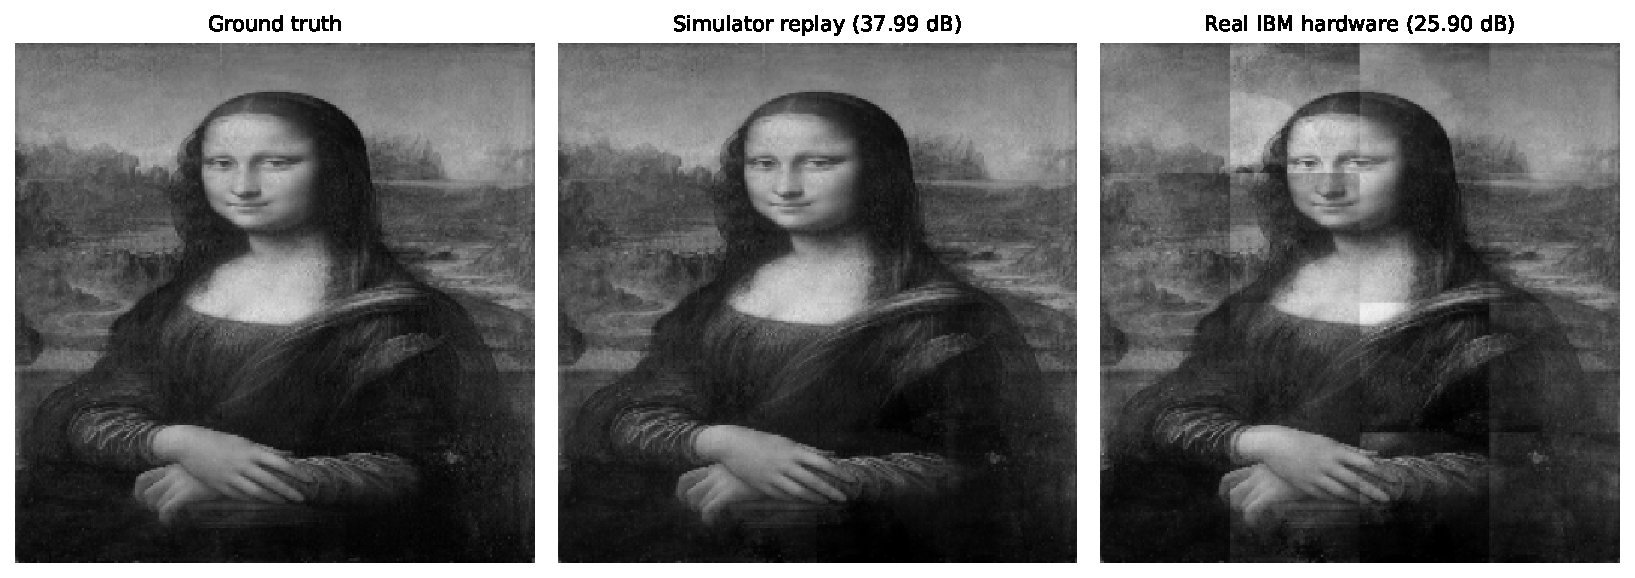
\includegraphics[width=\textwidth]{figures/ibm_hardware_reconstruction_monalisa.pdf}
  \caption{\textit{Monalisa} reconstructed from real IBM Quantum hardware
           measurements (right) against the same trained checkpoint's
           noiseless-simulator replay (center) and ground truth (left). The
           hardware image is visibly noisier and exhibits patch-boundary banding,
           while the subject remains recognizable.}
  \label{fig:hardware_reconstruction_monalisa}
\end{figure}

\begin{figure}[t]
  \centering
  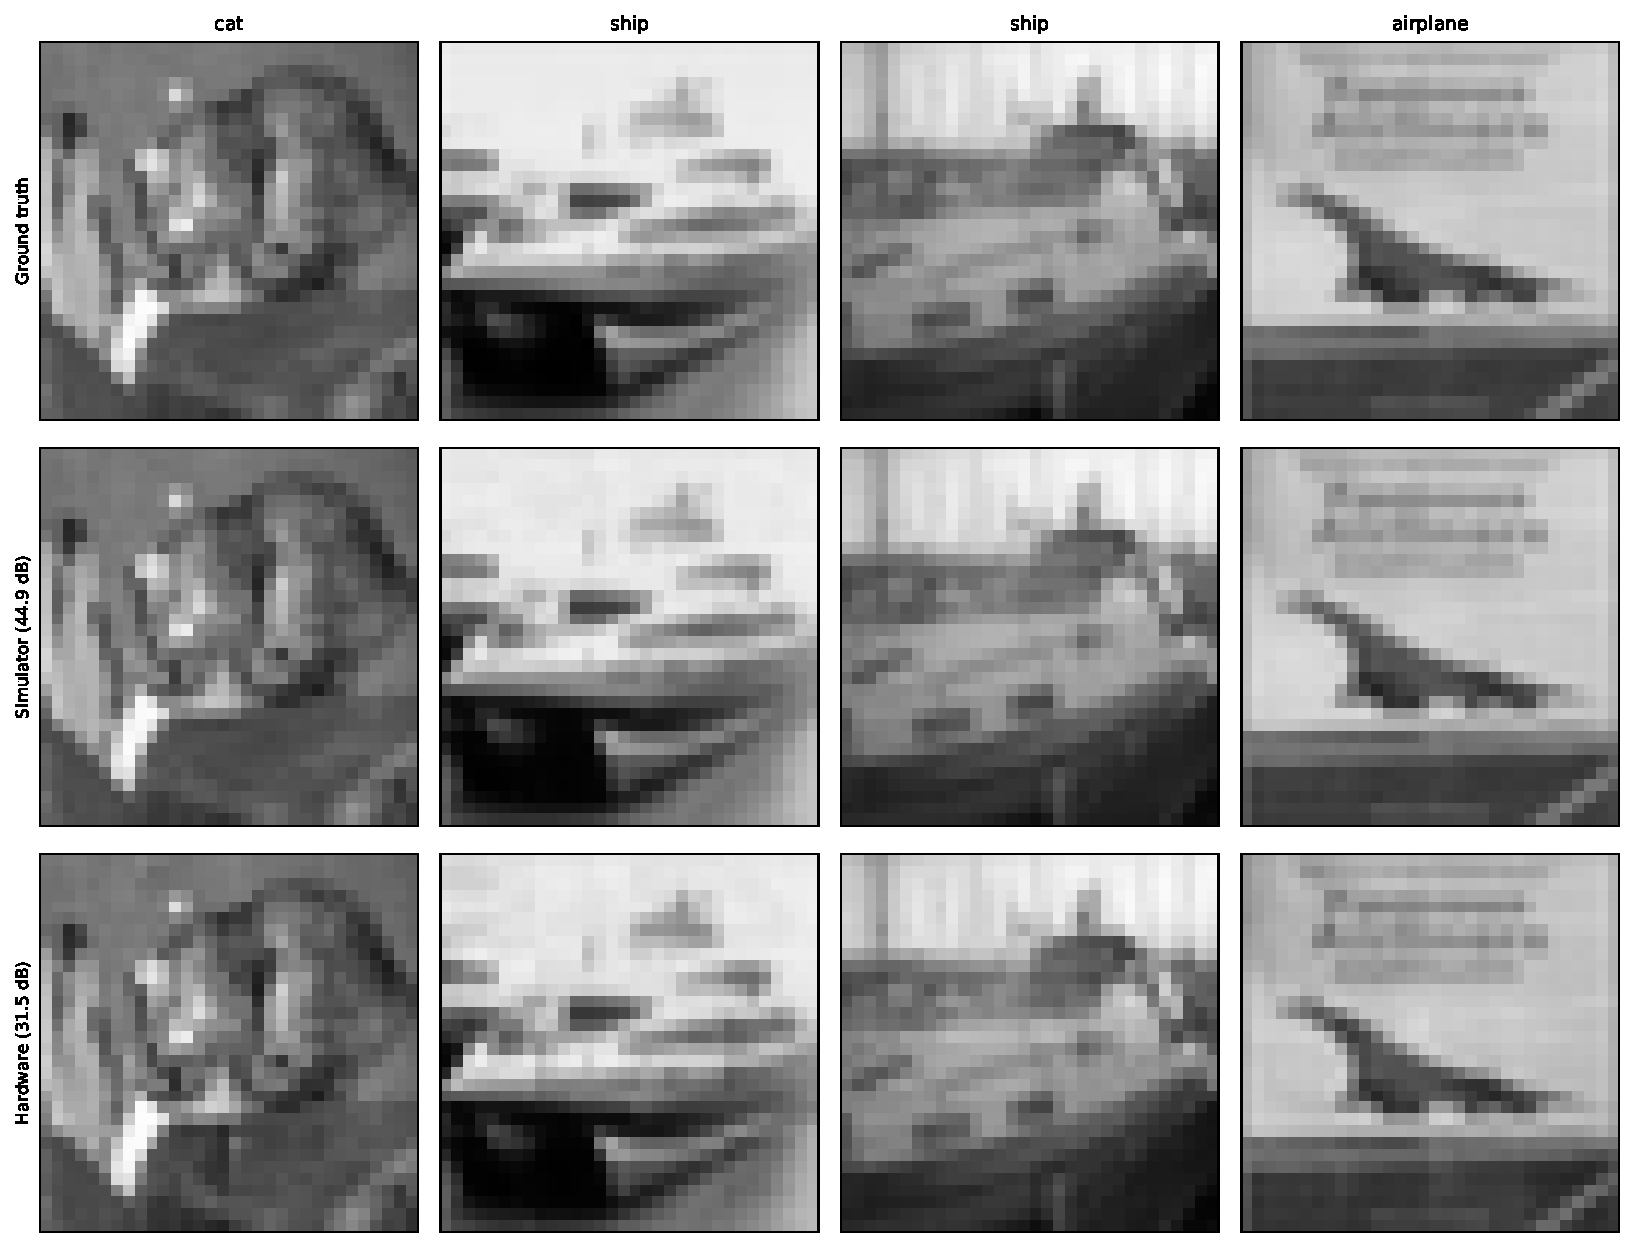
\includegraphics[width=\textwidth]{figures/ibm_hardware_reconstruction_cifar.pdf}
  \caption{Four CIFAR-10 images reconstructed from real IBM Quantum hardware
           measurements (bottom row) against noiseless-simulator replays of the
           same trained HVK2D checkpoints (middle row) and ground truth (top
           row).}
  \label{fig:hardware_reconstruction_cifar}
\end{figure}

Five images constitute a pilot, and we make no hardware-advantage claim. The
narrower result is that the trained HVK observable channel remains visually and
quantitatively informative in these device executions under the reported circuit
and shot budget. Full methodology --- exact gate sequences, per-basis measurement
construction, job IDs, and pre-submission local-validation results --- is
documented in the companion supplementary document.

The companion Supplementary Material reports a further hardware-validation
exercise built on this same checkpoint-replay methodology: fresh HVK1D
checkpoints trained at $N\in\{4,6,8\}$, replayed epoch-by-epoch on real IBM
Quantum hardware and on the IonQ cloud simulator \citep{IonQBackends}, in support
of the training-dynamics diagnostic discussed in
Section~\ref{sec:regularizer_inert} and the Supplementary Material. We keep it
out of the main text because it is a single-patch, single-seed probe in service
of a diagnostic whose own negative control (below) does not establish sensitivity
to the Hamiltonian term it is meant to track.

\subsection{Noise/shot trade-off: a free simulator complement}
\label{sec:hardware_robustness}

The five-image pilot above used a single shot budget (256/basis) and one
execution per image, which bounds how much it can say about noise sensitivity on
its own. Real IBM Quantum time is a scarce free-tier resource, so we separate
what a \emph{calibrated device-noise simulation} can establish at zero hardware
cost from what genuinely requires hardware. Using \texttt{qiskit-aer} with the
live calibration snapshot of \texttt{ibm\_fez} (\texttt{FakeFez}, no
quantum-processor time consumed), we replay the same already-trained
checkpoints' circuits at four shot budgets (256/512/1024/4096 shots per basis,
three repeated executions each) and compare against both the noiseless-simulator
ceiling and the real-hardware point already reported above.

\begin{figure}[t]
  \centering
  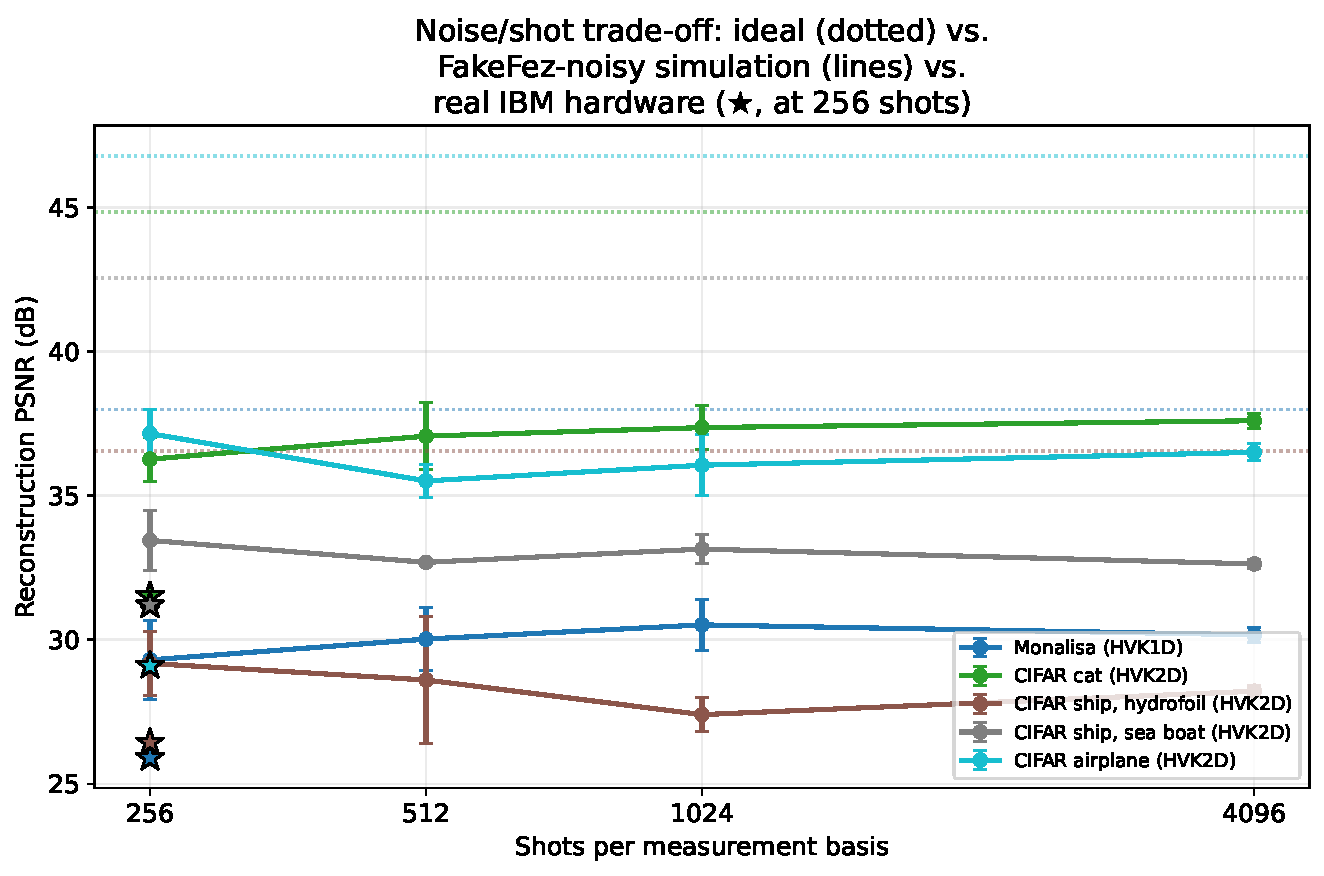
\includegraphics[width=0.85\textwidth]{figures/hardware_robustness_shot_sweep.pdf}
  \caption{Calibrated device-noise simulation (\texttt{FakeFez}, mean $\pm$ std
           over three executions). Dotted lines show noiseless ceilings and stars
           show real-hardware measurements. Increasing 256 to 4096 shots changes
           mean PSNR by only $-0.05$~dB.}
  \label{fig:hardware_robustness_shot_sweep}
\end{figure}

Two findings follow, averaged over the five checkpoints. First, shot noise
accounts for only part of the noiseless-to-real gap: moving from the noiseless
ceiling to a calibrated-noise simulation at the same 256-shot budget already
costs $8.68$~dB on average, before any real device is involved. Second, more
shots does not reliably recover it: increasing to 4096 shots per basis changes
PSNR by only $-0.05$~dB on average across the five checkpoints, with individual
images ranging from a $1.33$~dB gain to a $0.96$~dB loss. At this circuit size
and shot range, shot count is not a lever that reliably improves reconstruction
quality. Comparing the 256-shot noisy simulation directly against the
real-hardware point isolates what the calibration snapshot does \emph{not}
capture: a further $4.24$~dB average gap (range $2.25$--$8.06$~dB across images),
attributable to device effects a single calibration snapshot does not fully
capture --- drift between calibration and execution, crosstalk, and correlated
errors chief among them. The airplane image is the clear outlier ($8.06$~dB
residual gap, roughly double any other image), which we report rather than
exclude; a single-execution, five-image pilot cannot distinguish an
image-specific effect from ordinary job-to-job variation. This calibrated-noise
simulation is a free, repeatable complement to the pilot, not a substitute for
it: it bounds how much of the observed hardware gap is attributable to modeled
device noise versus unmodeled effects, using zero additional quantum-processor
time.

\subsection{Real-hardware anchor points: repeated execution and a second backend}
\label{sec:hardware_anchors}

The simulated trade-off above is bounded, in turn, by whether it actually
reflects real devices. We spent a small, explicitly quota-tracked slice of the
free-tier IBM Quantum allowance (four jobs, well under $1\%$ of the monthly
limit) confirming it directly: the same two checkpoints (\textit{Monalisa},
CIFAR \textit{cat}) replayed with no retraining on \texttt{ibm\_marrakesh} and
\texttt{ibm\_kingston} --- two backends distinct from the original pilot's
\texttt{ibm\_fez} --- at the original 256-shot budget and, separately, at 1024
shots.

\begin{table}[t]
  \centering
  \caption{Real-hardware anchor points: same checkpoints, no retraining, on two
           further backends. The original pilot's \texttt{ibm\_fez} point is
           shown for reference.}
  \label{tab:hardware_anchors}
  \begin{tabular}{@{}l l r r@{}}
    \toprule
    Image       & Backend                       & Shots & PSNR (dB) \\
    \midrule
    Monalisa    & \texttt{ibm\_fez} (original)  &  256  & 25.90     \\
    Monalisa    & \texttt{ibm\_marrakesh}       &  256  & 25.94     \\
    Monalisa    & \texttt{ibm\_kingston}        & 1024  & 26.10     \\
    \addlinespace
    CIFAR cat   & \texttt{ibm\_fez} (original)  &  256  & 31.52     \\
    CIFAR cat   & \texttt{ibm\_kingston}        &  256  & 28.93     \\
    CIFAR cat   & \texttt{ibm\_kingston}        & 1024  & 31.24     \\
    \bottomrule
  \end{tabular}
\end{table}

\textit{Monalisa} reproduces almost exactly across backends at matched shots
($25.94$ vs.\ $25.90$~dB, \texttt{ibm\_marrakesh} vs.\ \texttt{ibm\_fez}), and
gains only $0.16$~dB from quadrupling shots to 1024, consistent with the
simulated finding above that shot count is not a reliable lever. The CIFAR
\textit{cat} point is the more informative one: on \texttt{ibm\_kingston} at the
original 256-shot budget it reaches $28.93$~dB, $2.59$~dB below the
\texttt{ibm\_fez} pilot point, while its own 1024-shot execution on the same
backend recovers to $31.24$~dB, within $0.28$~dB of the original. This is real
job-to-job and backend-to-backend variation of a magnitude comparable to the
unmodeled residual identified by the simulator comparison
(Section~\ref{sec:hardware_robustness}). This is direct evidence, not merely a
simulated bound, that a single 256-shot execution on a single backend is not yet
a stable estimate of this pipeline's hardware performance, and that repeated
execution matters at least as much as backend choice or shot count individually.

\subsection{Exact \texorpdfstring{$D_4$}{D4}-equivariant observable pooling}
\label{sec:d4}
\label{sec:symmetry}

A $D_4$-pooled HVK2D observable-grid map is equivariant to the eight symmetries
of the square \emph{by construction}:
\begin{equation}
  \Phi_{D_4}(x)=\frac{1}{8}\sum_{g\in D_4}P_g^{-1}\Phi(gx),
  \qquad
  \Phi_{D_4}(hx)=P_h\,\Phi_{D_4}(x)\ \ \forall\, h\in D_4,
\end{equation}
up to floating-point error. We verify this numerically over 7000 patch transforms
of cached CIFAR images (Table~\ref{tab:d4_equivariance},
Figure~\ref{fig:d4_equivariance}): the pooled map's equivariance error is
$9.57\times10^{-17}\pm1.26\times10^{-17}$ (floating-point noise), while the
original unpooled positional map is not measurably more symmetric than a
local/raw control ($0.815\pm0.129$ vs.\ $0.837\pm0.131$) --- confirming the
unpooled map is only $D_4$-\emph{motivated} by the patch grid's geometry, not
empirically equivariant, and that only the explicit pooling construction delivers
the property. This is currently a feature-grid-level construction and numerical
diagnostic rather than a component of the trainable reconstruction pipeline;
integrating it end-to-end (Section~\ref{sec:limitations}) is concrete future
work.

\begin{table}[t]
  \centering
  \caption{$D_4$ equivariance error for unpooled and pooled observable-grid maps
           (lower is better; the pooled map is group-averaged over all eight
           square symmetries).}
  \label{tab:d4_equivariance}
  \begin{tabular}{@{}l r r@{}}
    \toprule
    Model                    & Mean error              & Std.\ error             \\
    \midrule
    $D_4$-pooled HVK2D       & $9.57\times10^{-17}$    & $1.26\times10^{-17}$    \\
    No positional encoding   & $7.40\times10^{-1}$     & $1.52\times10^{-1}$     \\
    HVK2D positional         & $8.15\times10^{-1}$     & $1.29\times10^{-1}$     \\
    Local/raw                & $8.37\times10^{-1}$     & $1.31\times10^{-1}$     \\
    \bottomrule
  \end{tabular}
\end{table}

\begin{figure}[t]
  \centering
  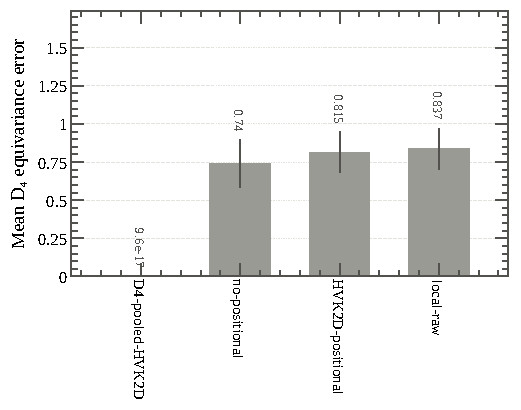
\includegraphics[width=0.85\textwidth]{figures/d4_equivariance_summary.pdf}
  \caption{$D_4$ equivariance diagnostic. The unpooled positional map is not
           equivariant; the group-pooled map is equivariant to numerical
           precision.}
  \label{fig:d4_equivariance}
\end{figure}

\subsection{Entanglement necessity in the nonlocal-structure protocol}
\label{sec:entanglement_necessity}

This diagnostic is deliberately constructed to reward pair-observable structure:
the target is a fixed synthetic function of \emph{simulated} patch features not
concatenated into any candidate's own input block (the companion supplement gives
the leakage-audit procedure that rules out circularity), and every control
receives the same raw inputs as HVK2D. Table~\ref{tab:hvk_pair_diagnostic} and
Figure~\ref{fig:hvk_pair_diagnostic} report the result across five seeds: HVK2D's
entangling observable channel reaches mean $R^2=0.9735$ ($32.77$~dB PSNR), a
$17.74$~dB improvement over a no-entanglement control ($R^2=0.019$) and
$18.52$~dB over random-VQC latents ($R^2=-0.173$); freezing the quantum circuit
(features fixed, only readout trained) still reaches $R^2=0.853$, while a
parameter-matched classical control ($R^2=-0.030$) and a frozen-classical control
($R^2=-0.903$) fail outright. The mechanism is explicit under the fixed linear
readout: a linear map of single-patch expectations $\{\langle O_i\rangle\}$ cannot
form the cross-term $\langle O_i\rangle\langle O_j\rangle$ that the target depends
on, whereas the entangling measurement supplies the joint correlator
$\langle O_iO_j\rangle$ directly as a feature. This is therefore evidence that an
entangling pair-observable channel is \emph{representationally necessary within
the tested feature class and fixed linear-readout protocol} to fit this target; a
sufficiently nonlinear classical readout could in principle recover the same
cross-terms, which is why we scope the claim to the linear protocol rather than to
classical models in general.

\begin{table}[t]
  \centering
  \caption{HVK2D restricted pair-correlation diagnostic across five seeds.
           Deliberately favorable to pair-observable structure; evidence for
           entanglement-necessity under a matched linear readout.}
  \label{tab:hvk_pair_diagnostic}
  \begin{tabular}{@{}l r r r@{}}
    \toprule
    Model                            & Mean MSE                  & Mean PSNR (dB) & Mean $R^2$ \\
    \midrule
    HVK2D entangling observables     & $8.5969\times10^{-4}$     & 32.77          & $ 0.9735$  \\
    Freeze quantum                   & $4.7904\times10^{-3}$     & 27.34          & $ 0.8533$  \\
    No entanglement                  & $3.1461\times10^{-2}$     & 15.03          & $ 0.0191$  \\
    Raw-linear classical             & $3.1654\times10^{-2}$     & 15.00          & $ 0.0133$  \\
    Parameter-matched classical      & $3.3033\times10^{-2}$     & 14.82          & $-0.0297$  \\
    Random VQC                       & $3.7616\times10^{-2}$     & 14.25          & $-0.1732$  \\
    Freeze classical                 & $6.0973\times10^{-2}$     & 12.17          & $-0.9025$  \\
    \bottomrule
  \end{tabular}
\end{table}

\begin{figure}[t]
  \centering
  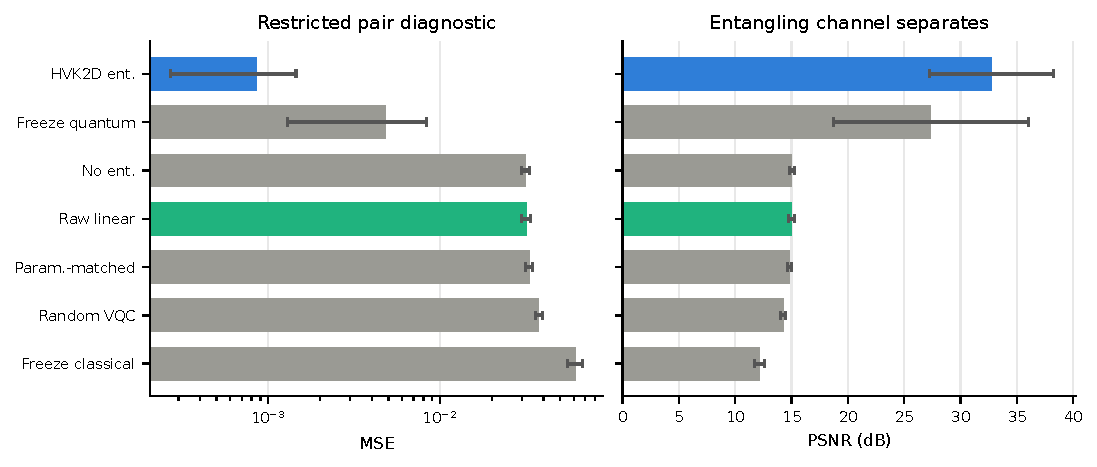
\includegraphics[width=0.9\textwidth]{figures/full_ablation_metric_comparison.pdf}
  \caption{Restricted pair-correlation diagnostic summary (mean $\pm$ std over
           five seeds). The entangling observable feature map dominates every
           control on this deliberately favorable task.}
  \label{fig:hvk_pair_diagnostic}
\end{figure}

\subsection{A scoped training-dynamics diagnostic}
\label{sec:phase_transition}

Beyond the results above, we tracked two exploratory training-dynamics readouts:
a magnetization-style statistic $M_z(t)$ and a signed energy-to-entanglement
ratio $R_{ES}(t)$. Neither exhibits a sharp transition: both drift smoothly
over training with run-to-run fluctuations, and any apparent onset is a
within-run median-plus-$2\sigma$ threshold crossing rather than a calibrated
statistical test. The negative control settles the reading: the identical
protocol applied to a classical-replacement variant, with the Hamiltonian energy
identically zero throughout training, crosses that threshold in all $4/4$ tested
cases --- exactly as often as the Hamiltonian-regularized model's $4/4$ --- so we
make no transition claim and report these traces solely as an interpretability
readout on the learned energy and entanglement (full protocol and tables in the
companion Supplementary Material).

\section{Discussion}
\label{sec:discussion}

\subsection{Why the physics-informed regularizer was inert}
\label{sec:regularizer_inert}

Table~\ref{tab:hamiltonian_controls} shows the Hamiltonian energy term is, if
anything, a mild drag on reconstruction quality in the present system. These are
fresh, same-environment measurements (\textit{Monalisa}, 200 steps, seed 42); an
earlier draft reported different absolute PSNR values for these same three
configurations, produced by a script that was never committed to the repository
and cannot be recovered or audited, so those earlier numbers are superseded here
rather than cited (full account of the discrepancy, plus additional
observable-sector controls and follow-up experiments, in the Supplementary
Material). The legacy objective adds a signed mean energy to the reconstruction
loss; because learned energy can go negative, the optimizer can lower total loss
by driving energy down without improving reconstruction, and removing the term
improves PSNR from $38.63$ to $44.56$~dB. Structurally, the learned couplings
enter only the energy term and never reach the decoder, so the Hamiltonian is a
\emph{read-only} observable of the trained representation rather than an inductive
bias on reconstruction; this is the precise sense in which we call it a diagnostic.
A contrastive variant --- assigning
lower energy to correct feature--position pairs than to shuffled pairs ---
improves over the signed-energy baseline ($42.92$~dB) but remains below its own
no-energy-loss counterpart ($44.56$~dB). We read this as a case where the
reconstruction loss already dominates the optimization signal at this model scale
and dataset size: a physically motivated regularizer has room to help when it
resolves an otherwise underdetermined objective, and here the pixel-fidelity loss
alone is sufficiently informative that the extra term mostly adds noise to the
gradient. This does not mean Hamiltonian regularization is never useful; its
value is conditional on the reconstruction loss being under-constrained, a
condition this patch-level pixel task does not meet. The Supplementary Material
additionally reports a root-cause fix (bounding the couplings and using a
positive/squared energy loss, which stops the term from hurting but does not make
it help) and an exploratory decoder-feature variant that improves 2 of 3 seeds
but regresses sharply on the third, too seed-sensitive to report as a validated
result here.

\begin{table}[t]
  \centering
  \caption{Hamiltonian-sector controls (single-seed, fresh same-environment
           reproduction: \textit{Monalisa}, 200 steps, seed 42). The energy
           objective is diagnostically useful but does not improve reconstruction
           accuracy. See the Supplementary Material for the full reproducibility
           investigation and additional observable-sector controls.}
  \label{tab:hamiltonian_controls}
  \begin{tabularx}{\textwidth}{@{}L{0.30\textwidth} c Y@{}}
    \toprule
    Experiment                      & PSNR (dB) & Interpretation \\
    \midrule
    Legacy baseline, signed energy  & 38.63     & Standard energy-regularized run \\
    No energy loss                  & 44.56     & Removing energy improves PSNR \\
    Contrastive Hamiltonian core    & 42.92     & Stronger objective helps modestly
                                                  vs.\ baseline, still below
                                                  no-energy-loss \\
    \bottomrule
  \end{tabularx}
\end{table}

The training-dynamics readouts of Section~\ref{sec:phase_transition} provide a
descriptive window into how the learned energy and entanglement evolve, and
nothing more: they are not calibrated statistical tests and must not be read as
thermodynamic transitions.

\subsection{Task-dependent representational scope}
\label{sec:dequant}
\label{sec:representativeness}

Whether a quantum feature map or kernel offers any advantage over a classical
model is a property of the specific data and target, not a fixed property of the
model class, and dequantization results have repeatedly shown that apparent
quantum advantages on structured, low-entanglement classical data can be matched
by classical algorithms once the right classical feature is identified
\citep{Huang2021PowerData, Tang2019}; where provable separations do exist, they
are established for carefully constructed learning problems rather than for
generic structured data \citep{Gyurik2023}. The restricted diagnostic of
Section~\ref{sec:entanglement_necessity} is constructed so that the relevant
structure is a genuine distant-element product raw or local features cannot
represent under a fixed linear readout, and that is precisely the regime in which
HVK's entangling channel separates. Natural image patches, at the resolution and
patch size used in ordinary reconstruction, are a different regime:
low-entanglement, locally structured data where a linear or shallow classical
readout is already close to sufficient. We stress that this is not a statement
about the circuit's entangling power: the ansatz uses strongly-entangling layers
and does generate an entangled state, but what the decoder consumes is the
\emph{measured pair-observable channel}, and whether that channel carries
task-relevant information is a property of the target, not of the circuit's
entanglement per se. On these natural-image targets the pair observables add
little beyond the local ones; on the constructed nonlocal target
(Section~\ref{sec:entanglement_necessity}) they are necessary. The companion supplementary study's
held-out comparisons (Section~\ref{sec:ablation_relationship}) characterize
exactly this second regime; together, the results delineate where the tested
entangling representation does and does not yield a measurable benefit.

This data-dependent reading also rules out an uncharitable alternative
explanation of the held-out tie (Section~\ref{sec:ablation_relationship}) and the
inert regularizer (Section~\ref{sec:regularizer_inert}): that some idiosyncratic
implementation choice --- an unmotivated qubit count, an unusual latent width, or
a peculiar regularizer formulation --- rather than the design pattern itself, is
responsible, and a different choice within the same pattern would have won. HVK's
three ingredients each recur individually throughout the hybrid quantum-vision
literature --- MPS compression of structured input
\citep{Stoudenmire2016, Han2018, Cirac2021, Guala2023}, a Pauli-correlator latent
space handed to a classical decoder \citep{Havlicek2019}, and a physically
motivated auxiliary regularizer alongside a task loss \citep{Shi2022} --- and its
specific instantiation (six-qubit VQC, $19$--$27$-D correlator vector,
graph-Hamiltonian term) sits well within the parameter ranges typical of that
literature rather than at an unusual extreme. The tested pattern is therefore a
fair, properly-scaled instance rather than a strawman, and its measured behavior
is evidence worth taking at face value; we do not, however, claim the boundary
transfers unchanged to every dataset, patch size, or qubit count.

\subsection{Topology alignment as an inductive bias}
\label{sec:topology}

Aligning the latent interaction graph with image-patch adjacency (HVK2D vs.\
HVK1D) is a plausible architectural inductive bias. The companion supplementary
study tests this hypothesis directly under matched held-out conditions. Its
real-circuit subset (3 seeds, 3 held-out CIFAR-10 images) gives an
HVK1D-minus-HVK2D mean PSNR difference of $0.16$~dB; after averaging images
within seed, the bootstrap 95\% CI is $[-0.38,0.46]$~dB and the seed-level
Wilcoxon test gives $p=0.50$. HVK2D completes the matched 90-step runs in roughly
half the wall-clock time. A broader five-seed surrogate comparison across
CIFAR-10, Fashion-MNIST, and PathMNIST likewise finds numerically small topology
differences (at most $0.07$~dB in mean PSNR). At the tested scale, topology
therefore appears to be primarily a resource-cost choice rather than a reliable
accuracy advantage; these tests do not establish formal equivalence.

Finally, Table~\ref{tab:differentiation} contrasts HVK's structural properties
against reference frameworks, including the three nearest hybrid-vision
architecture families discussed above (register-based QAE, quantum-kernel vision,
TN-circuit classifier). Its distinguishing features --- a Pauli-correlator latent
space, 2D Fourier positional bias with enforced $D_4$ pooling, and a Hamiltonian
energy diagnostic --- are documented and scoped in the preceding sections.

\begin{table}[t]
  \centering
  \caption{Architectural differentiation from representative baseline designs,
           including the three nearest hybrid-vision architecture families
           (register-based QAE, quantum-kernel vision, TN-circuit classifier).}
  \label{tab:differentiation}
  \scriptsize
  \setlength{\tabcolsep}{3pt}
  \begin{tabularx}{\textwidth}{@{}L{0.13\textwidth} Y Y Y Y Y Y@{}}
    \toprule
    Axis
      & Conv.\ AE baseline
      & GAN baseline
      & Register-based QAE
      & Quantum-kernel vision
      & TN-circuit classifier
      & HVK (ours) \\
    \midrule
    Latent representation
      & Continuous $\mathbb{R}^d$
      & Continuous $\mathbb{R}^d$
      & Quantum register
      & Scalar kernel value
      & MPS\slash circuit state
      & Pauli-correlator vector \\
    \addlinespace
    Spatial bias
      & Convolutional
      & Convolutional
      & Encoding-dependent
      & Encoding-dependent
      & MPS chain ordering
      & 2D Fourier encoding \\
    \addlinespace
    Auxiliary objective
      & Bottleneck / reconstruction
      & Adversarial loss
      & Fidelity / reconstruction
      & None (kernel value only)
      & Classification loss
      & Hamiltonian diagnostic \\
    \addlinespace
    Enforced group symmetry
      & Not in baseline
      & Not in baseline
      & Not in reference design
      & Not in reference design
      & Not in reference design
      & $D_4$ observable pooling \\
    \addlinespace
    Evaluated role
      & Reconstruction
      & Reconstruction
      & Compression
      & Classification
      & Classification
      & Reconstruction + diagnostics \\
    \bottomrule
  \end{tabularx}
\end{table}

\subsection{Validated scope and next steps}
\label{sec:limitations}

\begin{itemize}\itemsep4pt
  \item Every reconstruction result in this paper
        (Sections~\ref{sec:sameset_results}--\ref{sec:no_generalization}) is
        per-image trained, not held-out generalization; the companion
        supplementary study's held-out protocol is the appropriate evidence for a
        generalization claim, and its finding that local/raw maps match or exceed
        the tested HVK map under the shared readout should be read alongside the
        architecture-level results here.
  \item The $D_4$-pooled map (Section~\ref{sec:d4}) is currently a
        feature-grid-level construction and numerical diagnostic, not yet
        integrated into the trainable end-to-end reconstruction pipeline; doing
        so is concrete future work (Section~\ref{sec:conclusion}).
  \item The entanglement-necessity result
        (Section~\ref{sec:entanglement_necessity}) is scoped to a task
        deliberately constructed to require nonlocal structure; it does not by
        itself establish an advantage on ordinary natural-image reconstruction
        (see Section~\ref{sec:dequant}).
  \item The hardware pilot (Section~\ref{sec:hardware_pilot}) is a five-image,
        single-trial, unmitigated pilot, not a statistically resolved hardware
        benchmark.
  \item The training-dynamics traces (Section~\ref{sec:phase_transition}) are an
        interpretability readout, not evidence of a transition: the threshold's
        negative control fires on a classical-replacement variant with the
        Hamiltonian energy identically zero exactly as often as on the
        Hamiltonian-regularized model (4/4 vs.\ 4/4, full table in the
        Supplementary Material), so the readout has no demonstrated sensitivity
        to the Hamiltonian term itself.
  \item The matched real-circuit topology comparison uses only 3 seeds and 3
        held-out images per topology; the broader five-seed comparison is
        surrogate-based. These results support a resource-cost interpretation but
        do not establish formal equivalence of the topologies.
  \item Every result here is at a six-qubit, depth-18 scale. We therefore do not
        extrapolate these findings to wider circuits: the trainability of
        variational models is known to degrade with width and depth through
        barren-plateau effects \citep{McClean2018, Larocca2025}, so whether the
        tested boundary between HVK and resource-matched classical maps moves at
        larger scale is an open question this study does not answer.
\end{itemize}

\section{Conclusion}
\label{sec:conclusion}

We presented the Hamiltonian Vision Kernel, a new hybrid quantum--classical
architecture for image reconstruction that assembles matrix-product-state patch
features, a measured Pauli-correlator latent space, enforced $D_4$-equivariant
observable pooling, and a learnable Hamiltonian energy diagnostic into a single
pipeline --- a combination not previously assembled in this form
(Section~\ref{sec:representativeness}). Across six real image datasets,
per-image-trained HVK2D models reconstruct with high fidelity, and on a
resource-matched, multi-seed held-out comparison a pre-declared TOST equivalence
test shows HVK2D is \emph{competitive with}, rather than inferior or superior to,
simple classical controls (Section~\ref{sec:ablation_relationship}): local/raw
maps match or exceed it under the same fitted readout, and TOST confirms the gap
is small enough to call the two practically tied. We further reported a real IBM
Quantum hardware reconstruction pilot: replaying trained checkpoints without
retraining yielded $25.90$--$31.52$~dB PSNR from hardware measurements,
establishing feasibility at a five-image, single-trial scope rather than a
general hardware-performance claim.

If HVK ties classical baselines on ordinary reconstruction, its case rests on the
capabilities a purely classical reconstruction pipeline does not provide: a
restricted entanglement-sensitive result on a task requiring nonlocal structure,
where pair observables are necessary within the tested fixed-readout feature
class ($R^2=0.9735$ vs.\ $R^2\leq0.02$ for non-entangling controls), an
interpretable Hamiltonian energy diagnostic, and native execution on real quantum
hardware. Alongside these, the assembled pipeline is exactly $D_4$-equivariant by
construction (equivariance error $9.57\times10^{-17}$); we report that as a
design-correctness property rather than a quantum capability, since the same
Reynolds averaging applied to a classical feature map is equally exact. None of
these is in tension with the tie-with-classical result: entangling observables
separate only on the tested nonlocal target, and group pooling fixes equivariance
without by itself establishing an accuracy gain. We make no claim of quantum
advantage. HVK is, at this scope, a new architecture that works, is competitive
with resource-matched classical baselines, runs on real quantum hardware, and is
equipped with an entanglement-sensitive channel, an interpretable Hamiltonian
diagnostic, and native hardware execution --- capabilities a classical
reconstruction pipeline does not natively expose. We consider this carefully
measured boundary a constructive contribution alongside the architecture itself.

Future work should integrate the $D_4$-pooled map into an end-to-end trainable
pipeline (currently a feature-grid-level construction,
Section~\ref{sec:limitations}); scale the hardware pilot toward a statistically
resolved benchmark with error mitigation and repeated trials; search for further
real-world tasks with genuine nonlocal structure where HVK's restricted
entanglement-sensitive separation translates into a reconstruction advantage; and
extend the resource-matched, leakage-audited evaluation protocol used in the
companion supplementary study to other hybrid quantum vision architectures.

% ============================== BACK MATTER =================================
\backmatter

\bmhead{Supplementary information}

A companion document, \textit{Supplementary Material for the Hamiltonian Vision
Kernel: Resource-Matched Ablations, Validation, and Reproducibility}, accompanies
this manuscript.

\bmhead{Acknowledgements}

We thank the maintainers of the open-source scientific computing libraries used
in this work.

\section*{Statements and Declarations}

\begin{description}\itemsep4pt
  \item[Competing interests.] The authors declare no competing interests.

  \item[Funding.]``No funding was received for conducting this study.''

  \item[Data availability.] Dataset provenance and access routes are cited in the
        manuscript and detailed in the supplementary artifact map. All datasets
        used (CIFAR-10, MNIST, Fashion-MNIST, and the PathMNIST, BloodMNIST and
        PneumoniaMNIST subsets of MedMNIST~v2) are publicly available.

  \item[Code availability.] The source code, experiment drivers,
        machine-readable result summaries, validation arrays, and figure inputs
        supporting this study are included in the accompanying repository. The
        file \texttt{project\_artifacts/submission\_claim\_audit.json} maps each
        numerical headline claim to its retained source artifact --- including
        the resource-matched held-out comparison, on which the tested HVK map is
        competitive with rather than superior to the classical controls, and the
        withdrawn training-dynamics material --- and automated tests verify those
        mappings.
        IBM Quantum job identifiers and reconstructed outputs are retained; as
        disclosed in the supplement, the raw account-usage service response was
        not serialized, so the reported quota change is an execution-log record
        rather than a repository-recomputable measurement.

  \item[Author contributions.] \textbf{Sparsho Chakraborty:}
        Conceptualization, Methodology, Software, Validation, Formal analysis,
        Investigation, Data curation, Writing -- original draft, Visualization.
        \textbf{Siddhartha Patra:} Conceptualization, Supervision, Writing --
        review \& editing, Resources. Both authors reviewed and approved the
        final manuscript.
\end{description}

% ============================== REFERENCES ==================================
%  sn-jnl.cls sets the bibliography style from the sn-basic class option.
%  If BibTeX reports that it cannot open the style file, uncomment the next line.
% \bibliographystyle{sn-basic}
\bibliography{sn-bibliography}

\end{document}
